\chapter{Vícerozměrná lineární regrese}

Předpokládejme, že kromě $y_i$ máme pro~každé $i\in\widehat{n}$ k~dispozici také $m$ nezávislých proměnných $x_{i1},x_{i2},\dots,x_{im}$. Pak získáme model
 $$ Y_i = \beta_0+\sum_{j = 1}^m \beta_j x_{ij}+e_i,\quad i\in\widehat{n}, $$
kde $e_1,\dots,e_n$ jsou \textbf{nezávislé (nekorelované)} chyby a~$e_i\sim\NN(0,\sigma^2)$. Na~základě pozorování $(x_{i1},\dots,x_{im},y_i),~i\in\widehat{n}$ chceme odhadnout parametr $\betab = (\beta_0,\beta_1,\dots,\beta_m)^T$ (proložení dat \linebreak $m+1$ dimenzionální nadrovinou). Předpokládejme, že $n>m+1$, tj., že máme více dat než parametrů. Maticově můžeme tento stav zapsat jako
 $$ \Y = (Y_1,\dots,Y_n)^T,\quad \Y = (y_1,\dots,y_n)^T,\quad \eb = (e_1,\dots,e_n)^T. $$
Označme
 $$ \X = \left[\begin{array}{cccc}
1 & x_{11} &... & x_{1m} \\
1 & x_{21} &... & x_{2m} \\
1 & \vdots &... & \vdots \\
 \vdots& x_{n1} &... & x_{nm}
\end{array}
 \right] $$ jako \textbf{matici modelu} (regresní matici, \textit{design matrix}). Dostaneme tak model ve~tvaru (důležitém)
  \begin{equation}\label{the_chosen_one}
 \Y_{n\times 1} = \X_{n\times(m+1)}\betab_{(m+1)\times 1}+\eb_{n\times 1}. \tag{$**$}
 \end{equation}

 Nyní budeme předpokládat, že $e_1,\dots,e_n$ jsou nezávislé a~$e_i \sim\NN(0,\sigma^2)$, tzn. $\eb\sim\NN_n(\nula,\sigma^2 \In)$ a~$\Y\sim\NN_n(\X\betab,\sigma^2 \In)$.

 Věrohodnostní funkce je potom ve~tvaru
 \begin{align*}
 L(\betab,\sigma^2)& = f_\pi(\Y) = \prod_{i = 1}^n \frac{1}{\sqrt{2\pi\sigma^2}}\e{-\frac{1}{2\sigma^2}(y_i-\mu_i)^2} = \frac{1}{(2\pi\sigma^2)^{\frac{n}{2}}}\e{-\frac{1}{2\sigma^2}\sumin (y_i-\mu_i)^2} = \\ & = \frac{1}{(2\pi\sigma^2)^{\frac{n}{2}}}\e{-\frac{1}{2\sigma^2}(\Y-\boldsymbol{\mu})^T(\Y-\boldsymbol{\mu})} = \frac{1}{(2\pi\sigma^2)^{\frac{n}{2}}}\e{-\frac{1}{2\sigma^2}(\Y-\X\betab)^T(\Y-\X\betab)},
 \end{align*}
kde $\mu_i = \beta_0+\sumjn \beta_j x_{ij}$ a~$\boldsymbol{\mu} = (\mu_1,\dots,\mu_n)^T = \X\betab$.

 Pro~pevné $\sigma^2$ je
 $$ \max_{\betab} L(\betab,\sigma^2)\quad\Leftrightarrow\quad\min_{\betab}\underbrace{(\Y-\X\betab)^T(\Y-\X\betab)}_{g(\betab)} $$
 je opět pomocí derivací, ukážeme algebraický přístup.

\newpage
 \begin{theorem}
 	Uvažujme model \eqref{the_chosen_one} a~nechť $\eb\sim\NN(\nula,\sigma^2 \In)$. Potom $\wbetab$ je MLE $\betab$ právě tehdy, když $\wbetab$ je řešením soustavy rovnic
 	 $$ \X^T\X\betab = \X^T\Y\qquad\text{(soustava normálních rovnic)}. $$
 	Je-li matice $\X^T\X$ singulární, má tato soustava jednoznačné řešení ve~tvaru
 	 $$ \wbetab = (\X^T\X)^{-1}\X^T\Y. $$
 	\begin{proof}
 		\begin{enumerate}[$\Leftarrow$]
 			\item Ukážeme, že každé řešení $\wbetab$ soustavy $\X^T\X\betab = \X^T\Y$ minimalizuje $g(\betab)$ a~pro~každé $\betab$ platí, že
 			 $$ g(\bbeta) = \left((\Y-\X\betab)^T(\Y-\X\betab)\right) = \Y^T\Y-2\underbrace{\Y^T\X\betab}_{\wbetab^T\X^T\X}+\betab^T\X^T\X\betab = \Y^T\Y-2\wbetab^T\X^T\X\betab+\betab^T\X^T\X\betab $$
 			má platit i~pro~$\wbetab$ :
 			 $$ g(\wbetab) = \Y^T\Y-2\wbetab^T\X^T\X\wbetab+\wbetab^T\X^T\X\wbetab = \Y^T\Y-\wbetab^T\X^T\X\wbetab $$
 			a tedy
 			\begin{align}
 			g(\bbeta)-g(\wbetab)& = \betab^T\X^T\X\betab-2\wbetab^T\X^T\X\betab+\wbetab\X^T\X\wbetab = (\X\betab-\X\wbetab)^T(\X\betab-\X\wbetab) = \\
 			&= \left(\X(\betab-\wbetab) \right)^T\left(\X(\betab-\wbetab) \right) = \langle \X(\betab-\wbetab),\X(\betab-\wbetab) \rangle\geq 0,\quad\forall\betab, \label{tohle}
 			\end{align}
 			 tedy $\wbetab$ minimalizuje $g(\bbeta)$ a~je tedy MLE parametru $\betab$.
 		\end{enumerate}
 	\begin{enumerate}[$\Rightarrow$]
 		\item Předpokládejme, že $\wbetab_1$ minimalizuje $g(\betab)$ (je tedy MLE). To potom znamená, že \linebreak $g(\wbetab_1)\leq g(\betab),~\forall \betab$, speciálně $g(\wbetab_1)\leq g(\wbetab)$, kde $\wbetab$ je řešení soustavy $\X^T\X\betab = \X^T\Y$. Z~rovnice \eqref{tohle} vyplývá, že $g(\wbetab_1)\geq g(\wbetab)$. Celkem tedy $g(\wbetab_1) = g(\wbetab)$. Dosazením do~\eqref{tohle} dostaneme, že
 		 $$ 0 = g(\wbetab_1)-g(\wbetab) = \langle \X(\wbetab_1-\wbetab),\X(\wbetab_1-\wbetab) \rangle $$
 		a tedy $\X(\wbetab_1-\wbetab) = \nula$ Potom ale vynásobením $\X^T$ zleva dostaneme, že
 		 $$ \X^T\X\wbetab_1 - \underbrace{\X^T\X\wbetab}_{\X^T\Y} = 0\quad\Rightarrow\quad \X^T\X\wbetab_1 = \X^T\Y $$
 		 a~$\wbetab_1$ splňuje soustavu $\X^T\X\betab = \X^T\Y$.
 		
 		Aby byl důkaz korektní, je třeba ukázat, že soustava $\X^T\X\betab = \X^T\Y$ má vždy alespoň 1 řešení. Pokud existuje $(\X^T\X)^{-1}$, není co dokazovat, řešení máme přímo. Co když je ale $\X^T\X$ singulární?
 	\end{enumerate}
 	\end{proof}
 \end{theorem}
\begin{lemma}
	Soustava lineárních rovnic $\mathbb{A}\X = \Y$ má řešení právě tehdy, když $\langle \Y,\z\rangle = 0$ pro~všechna $\z$ splňující $\mathbb{A}\z = \nula$.
\end{lemma}
\begin{theorem}
	Soustava normálních rovnic $\X^T\X\betab = \X^T\Y$ má vždy alespoň jedno řešení.
	\begin{proof}
		Musíme ukázat, že $\langle \X^T\Y,\z\rangle = 0,~\forall\z$ splňující $\X^T\X\z = \nula$. Potom
		 $$\X^T\X\z = \nula~\Rightarrow~\langle \X^T\X\z,\z\rangle = \langle \X\z,\X\z\rangle = 0,$$ a~tedy $\X\z = \nula$. Celkem dostáváme $\langle\X^T\Y,\z\rangle = \langle\Y,\X\z\rangle = 0$. Obecně totiž platí, že $\langle \X,\mathbb{A}\Y\rangle = \langle \mathbb{A}^T\X,\Y\rangle$.
	\end{proof}
\end{theorem}
\begin{remark}
	Z vět vyplývá, že MLE $\betab$ může být nalezeno řešením $m+1$ lineárních rovnic o~$m+1$ neznámých. Málokdy existuje analytické řešení, je třeba použít numerické metody. Matice $\X^T\X$ může být v~praktických aplikacích špatně podmíněná, což ovlivňuje numerickou přesnost $\wbetab$. Proto se~často užívají metody jako Choleského rozklad, QR rozklad, singulární rozklad (SVD).
	
	Odvodili jsme to pro~normální chyby. Minimalizace $g(\betab)$ lze ale použít i~pro~jiné druhy chyb, potom se~$\wbetab$ nazývá \textbf{ordinary least squares estimate (OLS)} (obyčejné nejmenší čtverce). Asi nejužívanější metoda  pro~odhad $\betab$.
	
	Jak poznat, že mají normální rovnice jednoznačné řešení bez~nutnosti výpočtu $\X^T\X$?
\end{remark}
\begin{theorem}
	Matice $\X^T\X$ je nesingulární právě tehdy, když jsou sloupce matice $\X$ LN.
	\begin{proof}
		\begin{enumerate}[$\Leftarrow$]
			\item Sporem. Nechť jsou sloupce $\X$ LN a~matice $\X^T\X$ singulární, tzn. $\exists c\neq0$ tak, že $\X^T\X c = 0$. Potom
			 $$ 0 = \langle c,\X^T\X c\rangle = \langle \X c,\X c\rangle\quad \Rightarrow\quad\X c = 0,\qquad\sum c_i\X_i^c = 0, $$
			kde $c = (c_1,\dots,c_m)^T$ a~$\X_i^c$ je $i$-tý sloupec matice $\X$. Potom sloupce $\X$ jsou LZ. Spor.
		\end{enumerate}
	\begin{enumerate}[$\Rightarrow$]
	\item Sporem. Předpokládejme, že $\X^T\X$ je regulární a~sloupce $\X$ LZ. Potom existuje $c\neq0$ takové, že $\X c = 0$, $\X^T\X c = 0$. Z~toho vyplývá, že $\X^T\X$ je singulární. Spor.
\end{enumerate}
	\end{proof}
\end{theorem}
\begin{remark}
	Pokud $\X_{n\times(m-1)},~n>m+1,~h(\X) = m+1,~\eb\sim\NN(0,\sigma^2 I_m)$, pak existuje jednoznačné řešení normálních rovnic $\wbetab = (\X^T\X)^{-1}\X^T\Y$.
\end{remark}
\begin{remark}
	\begin{itemize}
		\item Pokud jsou sloupce $\X$ LZ, je $\X^T\X$ singulární, což je většinou detekováno numerickou metodou výpočtu $\wbetab$.
		\item Horší situace je, pokud jsou sloupce $\X$ \uv{téměř} LZ $\rightarrow$ tzv. \textbf{multikolinearita} -- způsobuje problémy při~výpočtu $\wbetab$, protože je $\x^T\x$ \uv{téměř} singulární. Jak ji detekovat probereme na~konci přednášky.
	\end{itemize}
\end{remark}

\section{Odhady parametrů}
\subsection{Odhad parametru $\sigma^2$ }
Pro normální chyby získáme MLE $\sigma^2$ derivací $\ln L(\beta, \sigma^2)$, z~čehož plyne:
\begin{align*}
	\hsn & = \frac{1}{n} \SSE = \frac{1}{n}(\y - \X \wbetab)^T(\y - \X \wbetab) = \frac{1}{n} \sumin (y_i - \hyi)^2, \\
	& \text{kde \;} \hyi = (\X \wbetab)_i = \x_i^T \wbetab, \quad i\in\widehat{n} \\
\end{align*}
a $\x_i^T$ značí i-tý řádek matice $\X$. Protože se~jedná o~vychýlený odhad, používá se~obecně odhad
 $$
	s_n^2 = \frac{1}{n-(m+1)} \SSE = \frac{1}{n - m - 1} \sumin (y_i - \hyi)^2
 $$
a $s_n = \sqrt{s_n^2}$ jako odhad $\sigma$ (už není nestranný).

Pro $e_i \sim \Nn$ se~také používají statistiky $s_n^2, s_n$.

\textit{Př. Ex. 5.13, str. 158 (nebo 138? jinak?)}

\textit{Ex. 5.15, str. 203}

\subsection{Vlastnosti odhadů $\wbetab, s_n^2$ }
\begin{theorem}
	Nechť $\wbetab$ je OLS odhad parametru $\betab$ v~modelu \eqref{the_chosen_one}, kde $h(\X) = m+1$ a~$e_1,\dots, e_n$ nezávislé, $e_i \sim (0,\sigma^2)$. Potom platí, že
	\begin{enumerate}
		\item $\E(\wbetab) = \betab$ (tj. $\wbetab$ je nestranný)
		\item $\Cov(\wbetab) = \sigma^2 (\X^T \X)^{-1}$
		\item $\E(s_n^2) = \sigma^2$
		\item Pokud navíc $e_i \sim \Nn, i\in\widehat{n} $, potom $\wbetab \sim \NN_{m+1}(\betab, \sigma^2(\X^T \X)^{-1})$. Speciálně $\wbeta_i \sim \NN(\beta_i, \sigma^2 \nu_i)$, kde $\nu_i$ je i-tý diagonání prvek matice $(\X^T \X)^{-1}$.
	\end{enumerate}
\end{theorem}

\begin{proof}
\begin{enumerate}
\item
\begin{align*}
	h(\X) & = m + 1 \Rightarrow \wbetab = (\X^T \X)^{-1} \X^T \Y \\
	\E \wbetab & = \E \left[(\X^T \X)^{-1} \X^T \Y \right] = (\X^T \X)^{-1} \X^T \E\Y = (\X^T \X)^{-1} \X^T \X \betab = \betab
\end{align*}

\item
Označíme vektor $\Y$ velikosti $(n \times 1)$ jako náhodný vektor, $\Cov(\Y) = \Sigma$. Pokud $\Am_{m, n}$ je matice, potom platí $\Cov(\Am \Y) = \Am \Sigma \Am^T$.

Protože $\wbetab = \Am \Y$, kde $\Am = (\X^T \X)^{-1} \X^T$, $\wbetab$ je LK $Y_1, \dots, Y_n$ a~$\Cov(\Y) = \sigma^2 \In$, tak
 $$
	\Cov \wbetab = (\X^T \X)^{-1} \X^T \sigma^2 \In \X (\X^T \X)^{-1} = \sigma^2 (\X^T \X)^{-1}.
 $$

\item
Nejdříve přepíšeme vektor reziduí $\heb = \Y - \X \wbetab = \Y - \hYb$. Pak
\begin{equation}
	\hYb = \X \wbetab = \X (\X^T \X)^{-1} \X^T \Y = \Hm \Y,
	\label{Eq: HY}
\end{equation}
kde $\Hm = \X (\X^T \X)^{-1} \X^T$ je tzv. \textbf{projekční matice}.
 
Pak $\heb = \Y - \Hm \Y = (\In - \Hm) \Y$. Dále platí
$$(\In - \Hm) \X = \X - \X (\X^T \X)^{-1} \X^T \X = \X - \X = \boldsymbol{0},$$
takže
 $$
	\heb = (\In - \Hm) \Y = (\In - \Hm)(\X \betab + \eb) = \underbrace{(\In - \Hm) \X}_{ = \boldsymbol{0}} \betab + (\In - \Hm) \eb = (\In - \Hm) \eb.
 $$
Zřejmě pak
\begin{align*}
& \Hm^T = \Hm \\
& \Hm^2 = \left[\X - \X (\X^T \X)^{-1} \X^T \right] \left[\X - \X (\X^T \X)^{-1} \X^T \right] = \X - \X (\X^T \X)^{-1} \X^T = \Hm \\
& (\In - \Hm)^2 = \In - \Hm
\end{align*}
tedy $\Hm$ je symetrická a~idempotentní. Spočítáme dále $\SSE$ jako
 $$
	\SSE = (\Y - \hYb)^T(\Y - \hYb) = \heb^T \heb = \heb^T (\In - \Hm)(\In - \Hm) \eb = \eb^T (\In - \Hm) \eb = \sumin \sumjn g_{ij} e_i e_j,
 $$
kde $g_{ij}$ je $(i,j)$-tý prvek matice $(\In - \Hm)$. Zbývá spočítat $\E(\SSE)$:

\begin{align*}
	\E(\SSE) & = \sumin \sumjn g_{ij} \underbrace{\E(e_i e_j)}_{\Cov(e_i, e_j)} = \left[\text{nekorelované, navíc\;} \E e_i = 0 \right] = \sumin g_{ii} \D e_i = \sigma^2 \sumin g_{ii} \\
	\sumin g_{ii} & = \trace(\In - \Hm) = \trace(\In) - \trace(\Hm) = n - \trace(\X (\X^T \X)^{-1} \X^T) = \\
	& = n - \trace(\X^T \X (\X^T \X)^{-1}) = n - \trace(\Identita{m+1}) = n - (m + 1)
\end{align*}

Celkem pak dostáváme $\E s_n^2 = \frac{1}{n - (m + 1)} \E (\SSE) = \frac{1}{n - (m + 1)} \sigma^2\left(n - (m + 1)\right) = \sigma^2$.

\item
 Jelikož $\wbeta$ je LK $Y_1,\dots, Y_n$, které jsou nezávislé a normálně rozdělené $$\Rightarrow \wbetab \sim \NN_{m+1} (\betab, \sigma^2(\X^T \X)^{-1}).$$
\end{enumerate}
\end{proof}

\begin{remark}
	Vlastnosti projekční matice:
	\begin{itemize}
		\item $\Hm = \X (\X^T \X)^{-1} \X^T, \quad \hYb = \Hm \Y, \quad \Hm^T = \Hm, \quad (\Identita{n} - \Hm)^T = (\Identita{n} - \Hm)$ -- symetrie
		\item $\Hm^2 = \Hm, \quad (\Identita{n} - \Hm)^2 = \Identita{n} - \Hm$ -- idempotentnost
		\item $\Hm \X = \X, \quad \trace(\Hm) = \sumin h_{ii} = m + 1$
		\item $\Hm(\Identita{n} - \Hm) = (\Identita{n} - \Hm) \Hm = \boldsymbol{0}$.
	\end{itemize}
\end{remark}

\begin{theorem}
	Nechť $\Y = \X \betab + \eb$ je LM \eqref{the_chosen_one}, kde $h(\X) = m + 1$ a~$\eb \sim \NN_n(\boldsymbol{0},\sigma^2 \Identita{n})$. Potom
	\begin{enumerate}
		\item $\wbetab$ a~$s_n^2$ jsou nezávislé náhodné veličiny,
		\item $(n - m - 1) \frac{s_n^2}{\sigma^2} \sim \chi^2(n - m - 1)$.
		\item Jestliže $v_i = (\X^T \X)_{ii}^{-1}$, potom $T_i = \frac{\wbeta_i - \beta_i}{s_n \sqrt{v_i}} \sim t(n-m-1)$.
		\item Nechť $\C \in \R^{r,m+1}$ takové, že $h(\eb) = r$. Potom kvadratická forma
		 $$
			\frac{q}{\sigma^2} = \frac{(\wbetab - \betab)^T \C^T \left[\C (\X^T \X)^{-1} \C^T \right]^{-1} \C (\wbetab - \betab)}{\sigma^2} \sim \chi^2(r).
		 $$
	\end{enumerate}
\end{theorem}

\begin{proof}
\begin{enumerate}
  \item Rozepíšeme
  $$ \wbetab = (\X^T \X)^{-1} \X^T \Y = (\X^T \X)^{-1} \X^T (\X \betab + \eb) = \betab + (\X^T \X)^{-1} \X^T \eb$$
a tedy $\wbetab - \betab = (\X^T \X)^{-1} \X^T \eb$. Dále víme, že $\heb = (\text{I}_n - \Hm) \eb$ a~vektor $(\wbetab - \betab, \heb)^T$ lze zapsat jako
 $$
\Zb \equal{\text{ozn.}} \left(\begin{array}{c}
 \wbetab - \betab \\
 \heb
\end{array}
 \right)
 = 
 \left(\begin{array}{c}
 (\X^T \X)^{-1} \X^T \\
 \text{I}_n - \Hm
 \end{array}
 \right) \eb
 = 
 \left(\begin{array}{c}
 \Am  \\
 \Bm
 \end{array}
 \right) \eb,
 $$
kde $\Zb$ je funkcí pouze $(e_1,\dots, e_n) = \eb \sim \NN (0, \sigma^2 \text{I}_n) \Rightarrow \Zb$ má vícerozměrné normální rozdělení (i~když degenerované, protože $\Cov(\Zb)$ je singulární, abychom ukázali, že $\wbetab$ a~$\heb$ jsou  nezávislé). \\
 ($s_n^2 = \frac{1}{n - m - 1} \heb^T \heb$, tedy i $\wbetab \text{ a~} s_n^2$ jsou nezávislé)
\begin{remark}
 $\Bm \Bm^T = \text{I}_n - \Hm \quad \text{je singulární, protože} \quad (\text{I}_n - \Hm) \X = 0$
\end{remark}
Stačí nám tedy ukázat, že $\Cov(\wbeta_i, \widehat{e}_j) = 0$ pro~$i = 0,\dots, m$ a~$j  \in\widehat{n} $ \\
spočtěme $\Cov(\Zb)$ : \\
 $$
  \Cov(\Zb)
 = 
  \left(\begin{array}{c}
 \Am  \\
 \Bm
 \end{array}
 \right) \Cov(\eb) \left(\Am^T \Bm^T  \right)
 = 
 \sigma^2
 \left(\begin{array}{c}
 \Am  \\
 \Bm
 \end{array} \right)
 \left(\Am^T \Bm^T  \right)
 = 
 \sigma^2
 \left(\begin{array}{cc}
 \Am \Am^T & \Am \Bm^T \\
 \Bm \Am^T & \Bm \Bm^T
 \end{array} \right)
 $$

 \begin{align*}
 \left(\Cov(\widehat{\beta}_i, \widehat{e}_j) \right)_{ \begin{array}{c}
 i = 0,\dots, m \\
 j  \in\widehat{n}
 \end{array} } & = \Am \Bm^T
 = (\X^T \X)^{-1} \X^T (\text{I}_n - \X (\X^T \X)^{-1} \X^T) = \\
& = (\X^T \X)^{-1} \X^T - (\X^T \X)^{-1} \X^T \X (\X^T \X)^{-1} \X^T = 0
 \end{align*}
 
\item Výsledky z~LA:
\begin{itemize}
\item $\Am_{n \times n}$ symetrická matice $\Rightarrow$ existuje ortogonální matice $\Qm$ a~diagonální matice $\Lam$ tak, že $\Am = \Qm \Lam \Qm^T$, sloupce $\Qm$ jsou ON vlastní vektory matice $\Am$ a~diagonální prvky matice $\Lam$ jsou jim odpovídající vlastní čísla.
\item $\Am_{n \times n}$ idempotentní matice $\Rightarrow$ vlastní čísla jsou pouze 0 nebo 1 $\Rightarrow h(\Am) = \trace(\Am)$.
\end{itemize}
V důkazu předchozí věty jsme ukázali, že
$$(n - m -1) \frac{s_n^2}{\sigma^2} = \frac{\SSE}{\sigma^2} = \frac{1}{\sigma^2} \eb^T (\text{I}_n - \Hm) \eb.$$
Protože je $(\text{I}_n - \Hm)$ symetrická a~idempotentní, tak
 $$
 \text{I}_n - \Hm = \Qm \Lam \Qm^T,  \quad \text{kde} \quad
 \begin{array}{c}
 {\Qm  \text{ je ortogonální matice}} \\
{\Lam  \text{ je diagonální matice s~vlastními čísly } \text{I}_n - \Hm}
 \end{array}.
 $$
Protože vlastní čísla $\text{I}_n - \Hm$ jsou 0 nebo 1 a~$\trace(\text{I}_n - \Hm) = h(\text{I}_n - \Hm) = n - m - 1$, \linebreak
 $\Lam$ může být zapsána ve~tvaru:
 $$
 \Lam = 
 \left(\begin{array}{cc}
 \textbf{I}_{n-m-1} & \nula  \\
 \nula & \nula
 \end{array} \right),
 $$
takže
 $$
 \eb (\text{I}_n - \Hm) \eb = \eb \Qm \Lam \Qm^T \eb = \qb^T \Lam \qb, \quad \text{kde } \qb = \Qm^T \eb.
 $$
 
\begin{theorem}
	 $\Vm \sim \NN_n (\nula, \In)$ a~$\Qm$ je ortogonální matice, potom $\Qm \Vm \sim \NN_n (\nula, \In).$
\end{theorem}
\vspace{0.1cm}
To znamená, že $\qb$ je vektor nezávislých $\NN(0,\sigma^2)$ veličin $\left(\qb \sim \NN_n (\nula, \sigma^2 \In)\right)$ a
 $$ \frac{1}{\sigma^2} \eb^T (\text{I}_n - \Hm) \eb = \frac{1}{\sigma^2} \qb^T \Lam \qb = \sum_{i = 1}^{n-m-1}\frac{q_i^2}{\sigma^2} \quad \sim \chi^2 (n - m - 1) $$
je suma druhých mocnin $n-m-1$ nezávislých $\NN(0,1)$ veličin.
\item Z~předchozí věty:
 $$
  \frac{\widehat{\beta}_i - \beta_i}{\sigma \sqrt{v_i}} \sim \NN(0,1) \quad \text{a} \quad \frac{s_n}{\sigma} = \sqrt{\frac{\frac{(n-m-1) s_n^2}{\sigma^2}}{n-m-1}} = \sqrt{\frac{\chi^2(n-m-1)}{n-m-1}}
 $$
a z~bodu $1)$ nezávislost
\begin{equation}
  \text{T}_i = \frac{\widehat{\beta}_i - \beta_i}{s_n \sqrt{v_i}} = \frac{\frac{\widehat{\beta}_i - \beta_i}{\sigma \sqrt{v_i}}}{\frac{s_n}{\sigma}} \sim \mathrm{t}(n-m-1)
\label{Rozdeleni_T}
\end{equation}
\item
 $\C \widehat{\beta} \sim \NN_r \left(\C \beta, \sigma^2 \C (\X^T \X)^{-1} \C^T \right)$, a~tedy
 $$ \C (\widehat{\beta} - \beta) = \C\widehat{\beta} - \C \beta \sim \NN_r \left(\nula, \sigma^2 \C (\X^T \X)^{-1} \C^T\right). $$
Stačí tedy ukázat, že pokud $\Zb \sim \NN_r (\nula, \Sigma)$, potom $\Zb^T \Sigma \Zb \sim \chi^2(r)$.

Protože $\Sigma$ je pozitivně definitní, existuje regulární matice $\Rm$ taková, že $\Sigma = \Rm\Rm^T$. Protože $\textbf{U} = \Rm^{-1} \Zb$, potom $\E \textbf{U} = \Rm^{-1} \E [\Zb] = 0$.

Dále
$$\Cov(\textbf{U}) = \Rm^{-1} \Sigma (\Rm^{-1})^T = \Rm^{-1} \Rm\Rm^T (\Rm^T)^{-1} = \textbf{I}_r,$$
 tedy $\textbf{U} \sim \NN_r (\nula, \textbf{I}_r)$, takže složky \textbf{U} jsou nezávislé $\NN(0,1)$ rozdělené náhodné veličiny. Pak
 $$ \Rm^T \Sigma^{-1} \Rm = \textbf{U}^T \Rm^T (\Rm^T)^{-1} \Rm^{-1} \Rm \textbf{U} = \textbf{U}^T \textbf{U} = \sum_i^r \text{U}_i^2 \sim \chi^2(r) $$
za $\Rm = \C (\widehat{\beta} - \beta)$ a~$\Sigma^{-1} = \frac{1}{\sigma^2} [\C (\X^T \X)^{-1} \C^T]^{-1}$.

\end{enumerate}
\end{proof}

\subsection{Vlastnosti vektoru reziduí $\heb$ }

\begin{theorem}
	Uvažujeme model $\Y = \X \betab + \eb$, kde $e_1,\dots, e_n$ jsou nekorelované a~$e_i \sim (0,\sigma^2)$. Nechť $\wbetab$ je OLS $\betab$ a~$\heb = \Y - \hYb$ je vektor reziduí. Potom platí, že

\begin{enumerate}
\item $\E [\heb] = \nula$,
\item $\Cov(\heb) = \sigma^2 (\In - \Hm)$,
\item pokud navíc $\eb \sim \NN_n (\nula, \sigma^2 \In)$, potom $\heb \sim \NN_n (\nula, \sigma^2 (\In - \Hm))$,
\item jestliže má model intercept, tj. $\beta_0 \neq 0$, potom $\sumin \widehat{e}_i = 0$,
\item $\sumin \widehat{e}_i \widehat{y}_i = 0$.
\end{enumerate}		
\end{theorem}

\begin{proof}
Ukázali jsme, že $\heb = (\In - \Hm) \eb$.
\begin{enumerate}
\item $$\E [\heb] = (\In - \Hm) \cdot \E [\eb] = (\In - \Hm) \cdot 0 = 0$$
\item $$\Cov(\heb) = (\In - \Hm) \Cov(\eb) (\In - \Hm)^T = \sigma^2 (\In - \Hm)$$
\item $\heb$ je LK složek $\eb  \Rightarrow  \heb \sim \NN_n (\nula, \sigma^2 (\In - \Hm))$
\item Soustava normálních rovnic $\X^T \X \betab = \X^T \y$ lze zapsat jako $\X^T (\y - \X \betab) = \nula$. Pro první rovnici musí platit
 $$
 \sumin x_{i1} \cdot (y_i - \x_i^T \betab) = 0,
 $$
kde pro model s interceptem je $x_{i1}$ vektor jedniček. Pro $\wbetab$ tedy platí
 $$
 0 = \sumin (y_i - \x_i^T \wbetab) = \sumin (y_i - \widehat{y_i}) = \sumin \he_i.
 $$
\item Z~předchozího bodu platí pro~OLS $\wbetab$
 $$
 \X^T (\y - \X \wbetab) = 0
 $$
a přenásobením zleva $\wbetab^T$ dostaneme
 $$
  0 = \wbetab^T \X^T (\y - \X \wbetab) = \widehat{y}^T (\y - \hy) = \hy^T \heb = \sumin \hy_i \he_i.
 $$
\end{enumerate}
\end{proof}
\begin{remark}
Použitím bodů 4. a~5. dostaneme (stejně jako u~jednorozměrné regrese)
$$
\sumin (y_i - \overline{y})^2 = \sumin (\widehat{y}_i - \overline{y})^2 + \sumin (y_i - \widehat{y}_i)^2
$$
tedy
$$
\SST = \SSR + \SSE.
$$
\end{remark}

\section{Gauss - Markov theorem}
Pro \textbf{normální chyby}, tj. $e_i~iid~\NN(0,\sigma^2)$, je OLS $\wbetab$ MLE, tzn. je eficientní MVVE parametr $\betab$.

Pro \textbf{chyby nenormální} ukážeme, že OLS $\wbetab$ je BLUE (best linear unbiased estimation) parametru $\betab$ (za jistých podmínek), ale mohou ale existovat lepší lineární vychýlené odhady nebo nelineární odhady.

\begin{define}
	Nechť $\betab$ je vektor regresních parametrů v~lineárním modelu (LM). Řekněme, že $\wbetab$ je \textbf{lineární odhad} $\betab$, jestliže každé $\beta_i$ je LK pozorování $Y_i, i\in\widehat{n} $, tedy
	 $$
		\wbeta_i = \sumjn a_{ij} Y_j \quad i = 0,\dots,m
	 $$
V maticovém zápisu
	 $$
		\betab = \Am \Y, \quad \text{kde } \Am = (a_{ij})
	 $$
pro $i = 0,\dots, m$ a~$j  \in\widehat{n} $.
\end{define}
\begin{remark}
 Pokud v~modelu $\Y = \X \betab + \eb$ platí $h(\X) = m+1$, potom OLS $\wbetab$ je lineární, neboť $\wbetab = (\X^T \X)^{-1} \X^T \Y$, kde $\Am = (\X^T \X)^{-1} \X^T$
\end{remark}
\begin{theorem}[Gauss-Markov]
	Uvažujeme model $\Y = \X \betab + \eb$, kde matice $\X$ má plnou hodnost, $e_i, i\in\widehat{n} $ jsou nekorelované a~$e_i \sim (0, \sigma^2)$. Potom OLS odhad $\wbetab$ je BLUE parametru $\betab$ (best linear unbiased estimation).
\end{theorem}
\begin{proof}
	Nechť $\wbetab = \Am \Y$ je lineární odhad $\betab$. Aby byl nestranný musí platit $\E [\wbetab] = \betab$, tzn. $$ \E [\Am \Y] = \Am \E [\Y] = \Am \X \betab = \betab, $$
	tedy $(\Am \X - \textbf{I}_{m+1}) \betab = 0$. Protože to musí platit $\forall \betab \in \R^{m+1}$, dostáváme $\Am \X - \textbf{I}_{m+1} = 0$, nebo ekvivalentně $\Am \X = \textbf{I}_{m+1}$.
	
	Spočteme kovarianční matici $\wbetab$
 $$
	\Cov(\wbetab) = \Cov(\Am \Y) = \Am \Cov(\Y) \Am^T = \Am \sigma^2 \In  \Am^T = \sigma^2 \Am \Am^T.
 $$
Zapišme $\Am$ ve tvaru $\Am = (\X^T \X)^{-1} \X^T + \textbf{D}$, kde \textbf{D} je rozdíl mezi~$\Am$ a~maticí pro~OLS odhad.
Pokud ukážeme, že pro~nestranný lineární odhad $\wbetab = \Am \Y$, který minimalizuje rozptyl, musí platit $\textbf{D} = \nula$, bude věta dokázána.

Dosazením dostaneme:
\begin{align*}
	\Cov(\wbetab) & = \sigma^2 \left((\X^T \X)^{-1} \X^T + \textbf{D}\right) \left((\X^T \X)^{-1} \X^T + \textbf{D}\right)^T = \\
& = \sigma^2 \left[(\X^T \X)^{-1} + \textbf{D} \X (\X^T \X)^{-1} + (\X^T \X)^{-1} \X^T \textbf{D}^T + \textbf{DD}^T \right]
\end{align*}
a z~podmínek nerovnosti
 $$
\Am \X = \left[(\X^T \X)^{-1} \X^T + \textbf{D}\right] \X = \textbf{I}_{m+1} + \textbf{D} \X = \textbf{I}_{m+1}  \Rightarrow  \textbf{D} \X = 0 \text{, a~tedy i~} \textbf{D}^T \X^T = \nula.
 $$
To znamená, že
 $$
\Cov(\wbetab) = \sigma^2 \left[(\X^T \X)^{-1} + \textbf{DD}^T\right]
 $$
a pro~diagonální prvky platí
 $$
\D [\widehat{\beta}_i] = \sigma^2 \left[v_i + \sumjn d_{ij}^2\right], \quad i = 0,\dots, m.
 $$
Protože $v_i \geq 0$ a~$\sumjn d_{ij}^2 \geq 0 \Rightarrow \D [\widehat{\beta}_i]$ je minimalizován volbou $\sumjn d_{ij}^2 = 0$, tj. $d_{ij} = 0, j\in\widehat{n}$, platí $\forall i = 0,\dots, m \Rightarrow \textbf{D} = \nula$ tzn. lineárně nestranný odhad $\wbetab$, který minimalizuje $\D [\widehat{\beta}_i]$, $i = 0,\dots, m$ je $\wbetab = (\X^T \X)^{-1} \X^T \Y$.
\end{proof}
\section{Testování modelu - tabulka ANOVA}
\subsection{Celkový F-test (overall F-test)}

\begin{itemize}
\item Zajímá nás, zda je model statisticky signifikantní, tj. zda alespoň jeden z~koeficientů $\beta_1,\dots, \beta_m$ je nulový.
\item Mohli bychom testovat jednotlivé koeficienty $\text{H}_0 : \beta_j = 0$ pomocí alternativy t-testu.
\item Celková chyba I. druhu by takto ale mohla být velká, pokud máme hodně proměnných. Museli bychom hodně snížit $\alpha$ pro~jednotlivé testy, což zvýší pravděpodobnost chyby II.~druhu (tzn. riziko akceptování nenulových koeficientů jako nulových, a~tedy vynechání významných proměnných z~modelu).
\item Navíc je zde problém multikolinearity (viz později), jejímž jedním efektem jsou velké standardní chyby dohadů. To může vést k~akceptování všech koeficientů jako 0, i~když je model celkově významný (uvidíme na~příkladu).
\end{itemize}

Bylo by dobré mít jednu statistiku pro~test
 $$
\text{H}_0 : \beta_1 = \beta_2 = ... = \beta_m = 0 \quad \times \quad \text{H}_1 : (\exists i\in \widehat{m}, \beta_i \neq 0).
 $$
ANOVA přístup pro~jednorozměrnou regresi naznačuje, že statistika
 $$
\text{F} = \frac{\frac{\SSR}{m}}{s_n^2}
 $$
by mohla být užitečná (vyplyne i~z~obecnějších přístupů k~testování později).

\textbf{Značení:}

Označíme $\lx_j = \frac{1}{n} \sumin x_{ij}$ jako průměr j-tého sloupce matice $\X$,
 $$
	\lX = \begin{pmatrix}
	\lx_0 & \lx_1 & \cdots & \lx_m \\
	\vdots & \vdots & & \vdots \\
	\lx_0 & \lx_1 & \cdots & \lx_m
	\end{pmatrix}_{n \times m+1} 
 $$
 a $(\X_c)_{ij}$ centrované matice regresorů, kde $(\X_c)_{ij} = x_{ij} - \lx_j$, $i\in\widehat{n}, j = 1,\dots, m$.

\begin{theorem}
	V modelu $\Y = \X \betab + \eb$, kde $e_i$ jsou nekorelované a~$e_i \sim \Nn$ pro~$i  \in\widehat{n} $ platí
	 $$
		\E \left[\frac{\SSR}{m} \right] = \sigma^2 + \frac{\betab^T(\X - \lX)^T(\X - \lX) \betab}{m} = \sigma^2 + \frac{\betab_s^T \X_c^T \X_c \betab_s}{m},
	 $$
	kde $\betab_s = (\beta_1,\dots, \beta_m)$.
\end{theorem}

\begin{proof}
	
\begin{align*}
	\hyi & = \wbeta_0 + \sumjm x_{ij} \wbeta_j \\
	\frac{\partial \SSE}{\partial \beta_0} & = \sumin \left(y_i - (\beta_0 + \sumjn x_{ij} \wbeta_j) \right) = 0 \Rightarrow \wbeta_0 = \ly - \sumjm \lx_j \wbeta_j
\end{align*}
Celkem pak $\hy_i - \ly = \sumjm (x_{ij} - \lx_j) \wbeta_j, \quad i\in\widehat{n} $ a~zapsáno maticově:
 $$
\hYb - \lYb = (\X - \lX) \wbetab, \quad \text{kde} \; \lYb = (\ly, \ly,\dots, \ly)_{1 \times n}^T,
 $$
protože první sloupec matice $\X - \lX$ je nulový. Potom
 $$
\SSR = \sumin (\hy_i - \ly)^2 = (\hYb - \lYb)^T(\hYb - \lYb) = \wbetab^T \underbrace{(\X - \lX)^T(\X - \lX)}_{\Am} \wbetab = \wbetab^T \Am \wbetab
 $$

\begin{theorem}
	Nechť $Z = \Y^T \Am \Y$ je kvadratická forma a~nechť $\E \Y = \bmu$ a~$\Cov \Y = \Sigma$. Potom platí, že
	 $$
		\E Z~ = \trace(\Am \Sigma) + \bmu^T \Am \bmu.
	 $$
\end{theorem}

Nejdříve zjednodušíme matici $\Am$ :
\begin{align*}
	\lX & = \frac{1}{n} \Bm \X, \; \text{kde} \; \Bm = \begin{pmatrix}
	1 & 1 & \cdots & 1 \\
	\vdots & \vdots & & \vdots \\
	1 & 1 & \cdots & 1
	\end{pmatrix} \quad \text{a tedy} \\
	& \X - \lX = \left(\Identita{n} - \frac{1}{n} \Bm \right) \X \quad \text{a} \quad (\X - \lX)^T = \X^T \left(\Identita{n} - \frac{1}{n} \Bm \right) \\
	& \Am = (\X - \lX)^T(\X - \lX) = \X^T \underbrace{\left(\Identita{n} - \frac{1}{n} \Bm \right)^2}_{\Identita{n} - \frac{2}{n} \Bm + \frac{\Bm^2}{n^2}} \X = \X^T \left(\Identita{n} - \frac{1}{n} \Bm \right) \X
\end{align*}

Dále rozepíšeme $\underbrace{\Am \Sigma}_{ = \Am \Cov \wbetab} = \sigma^2 \X^T \left(\Identita{n} - \frac{1}{n} \Bm \right) \X \left(\X^T \X \right)^{-1}$ a~spočítáme $\trace (\Am \Sigma)$ :

\begin{align*}
\trace (\Am \Sigma) & = \sigma^2 \trace \left[\X \left(\X^T \X \right)^{-1} \X^T \left(\Identita{n} - \frac{1}{n} \Bm \right) \right] = \sigma^2 \trace\left[\Hm - \frac{1}{n} \Hm \Bm \right] = \\
& = \sigma^2 \left[\trace \Hm - \lomn{1} \trace (\Hm \Bm) \right] = \sigma^2 \left[\underbrace{\trace \Hm}_{ = m+1} - \lomn{1} \underbrace{\trace \Bm}_{ = n} \right] = \sigma^2 m,
\end{align*}
jelikož víme, že $\Hm \X = \X$ a~$\jednab = (1,\dots, 1)^T$ je první sloupec $\X$, takže $\Hm \jednab = \jednab$, a~tedy $\Hm \Bm = \Bm$. Celkem tak dostáváme
 $$
\E \left(\frac{\SSR}{m} \right) = \lm \left(\sigma^2 m + \betab^T (\X - \lX)^T(\X - \lX) \betab \right) = \sigma^2 + \lm \betab^T (\X - \lX)^T(\X - \lX) \betab
 $$
Navíc platí $(\X - \lX) \betab = \X_c \betab_s$, protože první sloupec matice $\X - \lX$ je nulový vektor.
\end{proof}

\begin{remark}
Pokud $\betab_s$ = 0, potom $\E \left(\frac{\SSR}{m} \right) = \sigma^2 = \E s_n^2$, takže $\betab_s \neq 0$ implikuje, že $\E \left(\frac{\SSR}{m} \right) > \sigma^2$, tedy velké hodnoty $\FF = \frac{\SSR/m}{s_n^2}$ budou znamenat zamítnutí $H_0: \betab_s = 0$. Budeme proto potřebovat rozdělení $\FF$ za~platnosti $H_0$.
\end{remark}

\begin{theorem}
Nechť v~modelu $\Y = \X \betab + \eb$ \eqref{the_chosen_one} jsou $e_1,\dots, e_n $~iid~$\Nn$. Pokud $\betab_s = 0$, tj. $\beta_1 = \beta_2 = \cdots = \beta_m = 0$, potom
 $$
\FF \sim \FF(m, n - m -1).
 $$
\end{theorem}

\begin{proof}
V důkazu minulé věty jsme ukázali
 $$
\SSR = \wbetab^T \X^T \left(\Identita{n} - \lomn{1} \Bm \right) \X \wbetab = \hYb^T \left(\Identita{n} - \lomn{1} \Bm \right) \hYb
 $$
a potřebujeme rozepsat $\hYb$, použijeme rovnost \eqref{Eq: HY}:
 $$
\hYb = \Hm \Y = \Hm (\X \betab + \eb) = \Hm \left( \jednab \beta_0 + \X_v \betab_s + \eb \right) = \beta_0 \underbrace{\Hm \jednab}_{= \jednab} + \Hm \X_v \underbrace{\betab_s}_{= \nula} + \Hm \eb = \beta_0 \jednab + \Hm \eb
 $$

 $$
\SSR = (\beta_0 \jednab^T + \eb^T \Hm)\left(\Identita{n} - \lomn{1} \Bm \right) (\beta_0 \jednab + \Hm \eb) = \eb^T \Hm \left(\Identita{n} - \lomn{1} \Bm \right) \Hm \eb,
 $$
protože $\left(\Identita{n} - \lomn{1} \Bm \right) \jednab = 0$ a~$\left(\Identita{n} - \lomn{1} \Bm \right)$ je symetrická.

Dále platí $\Hm = \Hm^T, \Hm^2 = \Hm$ a~$\Hm \Bm = \Bm \Hm = \Bm$ (protože $\Hm \jednab = \jednab$) a~celkem tedy dostáváme
 $$
\SSR = \eb^T \underbrace{\left(\Hm - \lomn{1} \Bm \right)}_{\text{ozn.} \; \C} \eb = \eb^T \C \eb.
 $$
Pro matici $\C$ platí
\begin{align*}
\C^T & = \left(\Hm^T - \lomn{1} \Bm^T \right) = \left(\Hm - \lomn{1} \Bm \right) = \C \\
\C^2 & = \left(\Hm - \lomn{1} \Bm \right)\left(\Hm - \lomn{1} \Bm \right) = \Hm^2 - \lomn{1} \Hm \Bm - \lomn{1} \Bm \Hm + \frac{1}{n^2} \Bm^2 = \Hm - \lomn{2} \Bm + \lomn{1} \Bm = \Hm - \lomn{1} \Bm = \C,
\end{align*}
tedy $\C$ je symetrická a~idempotentní, a~proto
 $$
h(\C) = \trace(\C) = \trace \left(\Hm - \lomn{1} \Bm \right) = m + 1 - 1 = m.
 $$
Z věty o~spektrálním rozkladu plyne existence $\Q$ OG a~diagonální $\Lam$ tak, že
 $$ \C = \Q^T \Lam \Q = \Q^T \left(\begin{array}{cc}
\Identita{m}&\nula  \\
\nula& \nula
\end{array}
 \right)\Q, $$
která má vlastní čísla $0$ a~$1$, protože se~jedná o~idempotentní matici. Dále potom
 $$ \SSR = \eb^T\Q^T\left(\begin{array}{cc}
 \Identita{m}&\nula  \\
 \nula& \nula
 \end{array}
 \right)\underbrace{\Q\eb}_{\Zb\sim\NN(\nula,\sigma^2 \Identita{n})} = \Zb^T\left(\begin{array}{cc}
 \Identita{m}&\nula  \\
 \nula& \nula
 \end{array}
 \right)\Zb = \sum_{i=1}^m Z_i^2, $$
 kde $Z_i\sim\NN(0,\sigma^2)$ jsou nezávislé. Z~toho vyplývá, že
 $$ \frac{Z_i}{\sigma}\sim\NN(0,1)\qquad\text{a}\qquad\frac{\SSR}{\sigma^2}\sim\chi^2(m). $$
 To znamená, že
 $$ \frac{\frac{\SSR}{\sigma^2 m}}{\frac{(n-m-1)s_n^2}{\sigma^2}\frac{1}{n-m-1}} = \frac{\frac{\SSR}{m}}{s_n^2} = \FF\sim \FF(m,n-m-1), $$
 pokud ukážeme, že $\SSR$ a~$s_n^2$ jsou nezávislé. K~tomu ale stačí dokázat, že $\SSR$ je nezávislé na~reziduích $\he_i,~i\in\widehat{n}$.
 $$ \SSR = \eb^T\Hm\left(\In-\frac{1}{n}\Bm \right)\Hm\eb = \eb^T\Hm\underbrace{\left(\In-\frac{1}{n}\Bm\right)\left(\In-\frac{1}{n}\Bm\right)}_{ = \In-\frac{1}{n}\Bm}\Hm\eb = \textbf{w}^T\textbf{w}, $$
 kde $\textbf{w} = \left(\In-\frac{1}{n}\Bm\right)\Hm\eb\equiv \Km\eb$, $\heb = (\In-\Hm)\eb\equiv \Lm\eb$. Stačí tedy ukázat, že $\textbf{w}$ a~$\heb$ jsou nezávislé vektory. Víme, že
 $$ \binom{\textbf{w}}{\heb} = \binom{\Km}{\Lm} \eb, $$
 tzn. má vícerozměrné normální rozdělení. Rozepíšeme kovarianci jako
  \begin{equation}\label{rovnicka}
  \Cov\binom{\textbf{w}}{\heb} = \binom{\Km}{\Lm}\Cov\left[\eb\right](\Km^T,\Lm^T) = \sigma^2 \left(\begin{array}{cc}
  \Km\Km^T&\Km\Lm^T  \\
  \Lm\Km^T & \Lm\Lm^T
  \end{array}
  \right).
  \end{equation}
  Pokud je výraz $\Km\Lm^T$ z~rovnice \eqref{rovnicka} roven nule, pak jsou $\textbf{w}$ a~$\heb$ nezávislé.
  Pro~$\Km\Lm^T$ platí, že
 $$ \Km\Lm^T = \left(\In-\frac{1}{n}\Bm \right)\underbrace{\Hm(\In-\Hm)}_{\Hm-\Hm^2 = \nula} = \nula. $$
\end{proof}

 $\test{\FF>\FF_{1-\alpha}(m,n-m-1)}$

 \begin{remark}
 	Odvozeno pro~$e_i\sim\NN(0,\sigma^2)$, obecně se~používá, i~když to nevíme, pro~velké $n$ může být často zdůvodněno pomocí CLV.
 \end{remark}
\subsubsection{Tabulka ANOVA}
 $$ \begin{array}{l|cccc}
\text{Source}& \mathrm{df} & \mathrm{SS} & \mathrm{MS} & F \\\hline
\text{Regression} & m & \SSR & \MSR = \frac{\SSR}{m} & \frac{\MSR}{\MSE} \\
\text{Residual} & n-(m+1) & \SSE & \MSE = \frac{\SSE}{n-m-1} = s_n^2 &  \\
\text{Total} & n-1 & \SST &  &  \\\hline
&  & \RR^2 & \overline{\RR}^2 &
\end{array}
 $$
\subsection{Koeficient (vícenásobné) determinace $\RR^2$ }
 Podobně jako u~jednorozměrné regrese, lze F-test chápat jako test významnosti $\RR^2$, definovaného jako
 $$ \RR^2\equiv \frac{\SSR}{\SST} = 1-\frac{\SSE}{\SST}, $$
protože
 $$ F = \frac{\frac{\SSR}{m}}{\frac{\SSE}{n-m-1}} = \frac{n-m-1}{m}\left(\frac{\frac{\SSR}{\SST}}{\frac{\SSE}{\SST}} \right) = \frac{n-m-1}{m}\frac{\RR^2}{1-\RR^2}, $$
 což je rostoucí funkce $\RR^2$ (opět $\RR^2\in[0,1]$).
 \begin{remark}
 	 $\RR^2$ je možno zvětšovat přidáváním nových proměnných $x$, i~když jsou statisticky nevýznamné. (Pro $n$ LN proměnných $x$ a~$n$ pozorování dostaneme \uv{perfect fit}, tedy přeučení.) Vysvětlení:
 	 $$ \RR^2 = 1-\frac{\SSE}{\SST}, $$
 	kde $\SST$ je pevně dáno daty $y$, ale $\SSE$ může být snížena přidáním proměnných $x$. Minimalizujeme totiž $(\y-\X\betab)^T(\y-\X\betab)$ přes větší množinu $\betab$. To znamená, že $\frac{\SSE}{\SST}$ je nerostoucí funkce počtu proměnných, a~tedy $\RR^2$ je neklesající funkce počtu proměnných. Z~tohoto důvodu se~někdy definuje \textbf{upravený koeficient determinace} (\textit{adjusted coefficient of determination})
 	 $$ \overline{\RR}^2 = \RR_{adj}^2 = 1-\frac{\frac{\SSE}{n-m-1}}{\frac{\SST}{n-1}} = 1-\frac{n-1}{n-m-1}\frac{\SSE}{\SST}. $$
 	S rostoucím $m$ klesá $\SSE$, ale i~$n-m-1$, což dává určitou kompenzaci.
 \end{remark}
\section{IS a~t-testy pro~parametry}
\begin{itemize}
	\item Pokud se~model ukáže jako významný, bude nás zajímat, které koeficienty přispívají.
	\item Lze použít IS a~TH stejně jako u~jednorozměrné regrese.
	\item Výsledky jsou odvozeny pro~normální chyby.
	\item V~praxi se~používají i~pro~jiné typy chyb (za jistých předpokladů budou platit asymptoticky, lze je použít pro~velká $n$).
\end{itemize}
Pro konstrukci použijeme dokázanou vlastnost (viz \eqref{Rozdeleni_T}):
 $$ \Tstat_j = \frac{\wbeta_j-\beta_j}{s_n\sqrt{v_j}}\sim t(n-m-1),\quad\text{kde } v_j = (\X^T\X)_{jj}^{-1}. $$
Standardním postupem získáme $100(1-\alpha)$\% IS pro~$\beta_j$ ve~tvaru
 $$ \left(\wbeta_j-t_{1-\frac{\alpha}{2}}(n-m-1)s_n\sqrt{v_j},\wbeta_j+t_{1-\frac{\alpha}{2}}(n-m-1)s_n\sqrt{v_j} \right).$$
S jejich pomocí lze odvodit kritický obor pro t-test
 $$ \hypothesis{\beta_j = b_j}{\beta_j\neq b_j} $$
ve tvaru
 $$ \frac{|\wbeta_j-b_j|}{s_n\sqrt{v_j}}>t_{1-\frac{\alpha}{2}}(n-m-1).$$
Pro $b_j = 0$ dostaneme test významnosti $\beta_j$, tzn. $H_0:~\beta_j = 0$ zamítneme, pokud
 $$ \frac{|\wbeta_j|}{s_n\sqrt{v_j}}>t_{1-\frac{\alpha}{2}}(n-m-1). $$
\begin{remark}
	\begin{itemize}
		\item Pokud nejsou porušeny předpoklady modelu nebo není přítomna kolinearita, lze zvážit odstranění všech nevýznamných proměnných (dle t-testu).
		\item V~případě kolinearity, model může být významný (dle celkového F-testu), ale všechny nebo téměř všechny proměnné se~mohou jevit jako nevýznamné (dle t-testů).
		\item Naopak, pokud má model velký počet možných proměnných, některé proměnné se~mohou jevit významné, i~když jsou náhodným šumem.
		\item Při~použití t-testů je třeba být obezřetný.
	\end{itemize}
\end{remark}
\begin{example}
	5.26, str. 230 a~5.27, str. 231
\end{example}
\begin{remark}
	Statistiky $\FF,\RR^2$ a~T jsou užitečné pro~rozkrytí efektů jednoduchých proměnných, nemohou být ale používány úplně automaticky.
\end{remark}

\section{Obecná lineární hypotéza}
F-test a~t-testy jsou speciálním případem \textbf{obecné lineární hypotézy}
 $$ \hypothesiswide{\C\betab = \textbf{b}}{\C\betab\neq\textbf{b}}, $$
kde $\C\in\R^{r\times(m+1)}$ a~$h(\C) = r$, tzn. $r\leq m+1$. Rovnice $\C\betab = \textbf{b}$ reprezentuje $r$ lineárně nezávislých podmínek
 $$ \sum_{j = 0}^m c_{ij}\beta_j = b_i,\quad i = 1,\dots,r. $$
\begin{remark}
	Jak volit $\bb$ a $\C$:
	
	\begin{enumerate}[a)]
		\item Volba $\textbf{b} = (0,\dots,0)^T$ a~$ \C = \left(\begin{array}{c|cccc}
		0 & 1 & 0 &... & 0 \\\hline
		0 & 0 & 1 &  & \vdots \\
		\vdots& \vdots & \ddots & \ddots & 0 \\
		0 & 0 & \dots & 0 & 1
		\end{array}
		\right)_{m\times(m+1)} $ vede na~test
		 $$ H_0:~\C\betab = \nula\qquad\Leftrightarrow\qquad H_0:~\beta_1 = \beta_2 = ... = \beta_m = 0. $$
		\item Volba $\textbf{b} = 0$ a~$\C = (0,\dots,0,1,0,\dots,0)$ vede na~test
		 $$ H_0:~\beta_j = 0. $$
		\item V~modelu $Y = \beta_0+\beta_1x_1+\beta_2x_2+\beta_3x_3+\beta_4x_4+e$ chceme testovat zároveň, že $\beta_2 = 0$ a~$\beta_3 = \beta_4$. To lze udělat volbou $ \C = \left(\begin{array}{rrrrr}
		0 & 0 & 1 & 0 & 0 \\
		0 & 0 & 0 & 1 & -1
		\end{array}
		 \right),~\textbf{b} = (0,0)^T $.
	\end{enumerate}
\end{remark}

Pro test $H_0$ naladíme 2 modely:\begin{description}
\item[plný model (full model)] bez~podmínek na~$\C\betab$,
\item[redukovaný model (reduced model)] za~předpokladu, že platí $H_0:~\C\betab = \bb$.
\end{description}

Označme příslušné reziduální součty čtverců $\SSE_F$ a~$\SSE_R$ (bude platit $\SSE_F\leq\SSE_R$).

\begin{itemize}
	\item Pokud neplatí $H_0$, dá se~očekávat, že $\Delta\SSE = \SSE_R-\SSE_F$ bude významně větší, než náhodná chyba $\sigma^2$, $H_0$ tedy budeme zamítat, pokud $\frac{\Delta\SSE}{s_n^2}$ bude velké.
	\item Zobecnění F-testu, tj. za~platnosti $H_0$ ukázeme pro~normální chyby vztah
	 $$ F = \frac{\frac{\Delta\SSE}{r}}{s_n^2}\sim\FF(r,n-m-1). $$
\end{itemize}
\begin{example}
	Uvažujme F-test pro~$H_0:\beta_1 = \beta_2 = ... = \beta_m = 0$ v~plném modelu. Redukovaný model bude $Y_i = \beta_0+e_i,~i = 1,\dots,n~\Rightarrow~\wbeta_0 = \overline{\y}$ a~$\SSE_R = \sumin (y_i-\ly)^2 = \SST$, tedy
	 $$ \Delta \SSE = \SST-\SSE_F = \sumin (y_i-\ly)^2-\sumin (y_i-\hy_i)^2 = \SSR $$
	 a~statistiku $F = \frac{\frac{\SSR}{m}}{s_n^2} = F_{overall}\sim\FF(m,n-m-1)$, jak jsme již ukázali.
\end{example}
\begin{theorem}
	Nechť v~modelu \eqref{the_chosen_one} platí, že $e_1,\dots,e_n$ jsou nezávislé a~$e_i\sim\NN(0,\sigma^2)$. Označme $\SSE_F$ reziuální s.č. plného modelu a~$\SSE_R$ reziduální s.č. modelu, kde platí $H_0:~\C\betab = \textbf{b}$. Potom je za~platnosti $H_0$ splněno
	 $$ F = \frac{\frac{\Delta\SSE}{r}}{s_n^2}\sim\FF(r,n-m-1). $$
\end{theorem}
\begin{proof}

\newcommand{\yb}{\boldsymbol{y}}
\newcommand{\lambdab}{\boldsymbol{\lambda}}
\newcommand{\xtx}{(\X^T \X)^{-1}}
\newcommand{\parcialni}[2]{\frac{\partial #1}{\partial #2}}

Nejdříve si dokámeme následující lemma:
\begin{lemma}
	Označme $\wbetab_F$ a~$\wbetab_R$ LSE parametru $\betab$ v~plném a~redukovaném modelu. Potom platí
	\begin{enumerate}
		\item $\wbetab_F = \wbetab_R - (\X^T \X)^{-1} \C^T \Am (\C \wbetab_F - \bb)$, kde $\Am = \left(\C (\X^T \X)^{-1} \C^T \right)^{-1}$
		\item $\Delta \SSE = \SSE_R - \SSE_F = \left(\C \wbetab_F - \bb \right)^T \Am \left(\C \wbetab_F - \bb \right)$.
	\end{enumerate}
\end{lemma}

\begin{proof}
\begin{enumerate}
\item
Víme, že $\wbetab_F = \xtx \X^T \yb$ a~musíme najít $\wbetab_R$. Budeme proto minimalizovat
 $$
g(\betab) = (\yb - \X \betab)^T(\yb - \X \betab)
 $$
za podmínky $\C \betab = \bb$. Sestavíme Lagrangeovu funkci
\begin{align*}
L & = L(\betab) = g(\betab) - 2 \lambdab^T(\C \betab - \bb), \; \text{kde} \quad \lambdab = (\lambda_1,\dots, \lambda_r) \\
L & = \yb^T \yb - 2 \yb^T \X \betab + \betab^T \X^T \X \betab - 2 \lambdab^T \C \betab + 2 \lambdab^T \bb
\end{align*}
a tedy
\begin{align*}
\frac{\partial L}{\partial \betab} & = \left(\parcialni{L}{\beta_0}, \parcialni{L}{\beta_1},\dots, \parcialni{L}{\beta_m} \right)^T = 2 \X^T \X \betab - 2 \X^T \yb - 2 \C^T \lambdab = 0 \\
\parcialni{L}{\lambdab} & = \left(\parcialni{L}{\lambda_1},\dots, \parcialni{L}{\lambda_r} \right)^T = \C \betab - \bb = 0.
\end{align*}
Z první rovnice dostáváme
\begin{equation}
\wbetab_R = \xtx \X^T \yb + \xtx \C^T \lambdab = \wbetab_F + \xtx \C^T \lambdab \tag{+} \label{Eq: Lagrange prvni}
\end{equation}
a dosadíme do~druhé
 $$
\C \wbeta_R - \bb = \C \wbetab_F - \bb + \C \xtx \C^T \lambdab = 0.
 $$
Můžeme tak spočítat $\lambdab = -\left(\C \xtx \C^T\right)^{-1} \left(\C \wbetab_F - \bb \right)$ a~dosazením do~rovnice \eqref{Eq: Lagrange prvni} získáme
 $$
\wbetab_R = \wbetab_F - \xtx \C^T \left(\C \xtx \C^T \right)^{-1} \left(\C \wbetab_F - \bb \right) = \wbetab_F - \xtx \C^T \Am (\C \wbetab_F - \bb).
 $$

\item
Z důkazu věty $\wbetab = \xtx \X^T \y$ víme, že
 $$
g(\betab) - g(\wbetab_F) = (\betab - \wbetab_F)^T \X^T \X (\betab - \wbetab_F) \quad \forall \betab.
 $$
Dosadíme $\betab = \wbetab_R$ :
\begin{align*}
	\Delta \SSE & = g(\wbetab_R) - g(\wbetab_F) = (\wbetab_R - \wbetab_F) \X^T \X (\wbetab_R - \wbetab_F) = \\
	& = (\C \wbetab_F - \bb)^T \Am^T \C \xtx \X^T \X \xtx \C^T \Am (\C \wbetab_F - \bb) = (\times),
\end{align*}
a protože $\Am^T = \Am$, platí $\Am^T\underbrace{\C \xtx \C^T}_{ = \Am^{-1}} \Am = \Am \Rightarrow (\times) = (\C \wbetab - \bb)^T \Am (\C \wbetab - \bb)$.

\end{enumerate}
\end{proof}


Vrátíme se tedy k původnímu důkazu věty. Nejdříve ukážeme, že $\frac{\Delta \SSE}{\sigma^2} \sim \chi^2 (r)$ za platnosti $H_0: \C\betab = \bb$.

Za $H_0$ : $\Y \sim \NN(\X \betab_R, \sigma^2 \Identita{n})$ a~$\wbetab_F = \xtx \X^T \Y$, tzn.
 $$
\widehat{\boldsymbol{r}} = \C \wbetab_F - \bb \sim \NN\left(\E(\widehat{\boldsymbol{r}}), \Cov(\widehat{\boldsymbol{r}}) \right).
 $$
\begin{align*}
\E \widehat{\boldsymbol{r}} & = \E (\C \wbetab_F - \bb) = \E \left(\C \xtx \X^T \Y \right) - \bb = \C \xtx \X^T \E \Y - \bb = \\
& = \C \xtx \X^T \X \betab_R - \bb = \C \betab_R - \bb = 0 \quad \text{za platnosti \;} H_0 \\
\Cov(\widehat{\boldsymbol{r}}) & = \C \Cov(\wbetab_F) \C^T = \sigma^2 \C \xtx \C^T = \sigma^2 \Am^{-1} \\
& \Rightarrow \widehat{\boldsymbol{r}} = \C \wbetab_F - \bb \sim \NN \left(0, \sigma^2 \Am^{-1} \right)
\end{align*}
Tedy
 $$
\frac{\Delta \SSE}{\sigma^2} = \frac{\widehat{\boldsymbol{r}}^T \Am \widehat{\boldsymbol{r}}}{\sigma^2} \sim \chi^2(r).
 $$

Navíc bod 4) věty na~str (55), kde $\Zb \sim \NN_r(0, \Sigma) \Rightarrow \Zb^T \Sigma^{-1} \Zb \sim \chi^2(r)$ a~bod 1) $\Rightarrow \wbetab_F$ a~$s_n^2$ jsou nezávislé.

Tedy $\Delta \SSE$ je funkcí pouze $\wbetab_F$, tzn nezávisí na~$s_n^2$, takže
 $$
F = \frac{\frac{\Delta \SSE}{\sigma^2 r}}{\frac{(n-m-1)s_n^2}{\sigma^2(n-m-1)}} = \frac{\frac{\Delta \SSE}{r}}{s_n^2} \sim F(r, n-m-1).
 $$
\end{proof}

\begin{remark}
Použitím rozkladu $\SST = \SSE + \SSR$ dostaneme
 $$
\Delta \SSE = \SSR_F - \SSR_R.
 $$
Interpretace: nárůst regresního součtu čtverců díky~neplatnosti $H_0$. Dále
 $$
\SSR_F = \SSR_R + \Delta \SSE,
 $$
kde $\Delta \SSE$ je \textit{extra sum of squares} přidaná k~$\SSR$ díky~neplatnosti $H_0$.

Např., pokud $\betab = (\beta_0, \beta_1,\dots, \beta_{m-1}, 0)$, tzn. $\beta_m = 0$ a~skutečný model má $\betab = \betab_F$, potom $\Delta \SSE$ je extra regresní součet čtverců získaný díky~přidání $\beta_m$ do~modelu.

Umožňuje rozklad $\SSR$ plného modelu na~jednotlivé části $\left(x_1, x_2 | x_1, x_3 | x_2 x_1,... \right)$.
\end{remark}

Př. analogie k~Př. 5.25 str. 238

\begin{remark}
	Joint confidence region viz. Ex 5.30 str. 239
\end{remark}



\section{Predikce}
Jakmile máme adekvátní model, můžeme ho použít pro~bodové a~intervalové predikce jako u~jednorozměrné regrese.

\begin{description}
	\item[a) predikce] $\E [Y_{\x_0}]$

Nechť $\x_0 = (1, x_{0,1},\dots, x_{0,m})^T$ je nový bod proměnné $\x$. Bodový odhad $\E [Y_{\x_0}]$ je roven
 $$
 \widehat{y}_{\x_0} = \widehat{\beta}_0 + \sum_{j = 1}^m x_{0,j} \widehat{\beta}_j = \x_0^T \wbetab
 $$

tzn. $\D [\hY_{\x_0}] = \x_0^T \cdot \D [\widehat{\betab}] \cdot \x_0 = \sigma^2 \x_0^T(\X^T \X)^{-1} \x_0$ a~může být odhadnut pomocí
 $$
 \widehat{\sigma}^2(\hY_{\x_0}) = s_n^2 [\x_0^T(\X^T \X)^{-1} \x_0] \quad \text{(rozptyl predikce)}.
 $$
 Speciálně pokud $\x_0^T = \x_i^T$ ($i$-tý řádek matice $\X$), tak
 $$
  \widehat{\sigma}^2(\hY_{\x_i}) = s_n^2 [\x_i^T(\X^T \X)^{-1} \x_i] = s_n^2 h_{ii}, \quad \text{kde } h_{ii} = (\Hm)_{ii} \quad \text{a} \quad \Hm = \X (\X^T  \X)^{-1} \X^T.
 $$
Pro normální chyby lze odvodit interval spolehlivosti pro~$\E [Y_{\x_0}] = \mu_{\x_0}$, protože $\hY_{\x_0}$ je LK náhodné veličiny s~vícerozměrným normálním rozdělením. Proto má normální rozdělení s $\E [\hY_{\x_0}] = \mu_{\x_0} = \x_0^T \betab$ a~$\D [\hY_{\x_0}] = \sigma^2 \x_0^T(\X^T \X)^{-1} \x_0$
tzn.
 $$
\frac{\hY_{\x_0} - \mu_{\x_0}}{\sigma \sqrt{\x_0^T(\X^T \X)^{-1} \x_0}} \sim \NN(0,1)
 $$
a díky~nezávislosti $\wbetab$ a~$s_n^2$
 $$
 \frac{\hY_{\x_0} - \mu_{\x_0}}{s_n \sqrt{\x_0^T(\X^T \X)^{-1} \x_0}} \sim \mathrm{t}(n-m-1)
 $$
 čímž získáme $100(1-\alpha)\%$ interval spolehlivosti pro $\mu_{\x_0}$
 $$
   (\hY_{\x_0} \pm \mathrm{t}_{1-\frac{\alpha}{2}}(n-m-1) \cdot s_n \sqrt{\x_0^T(\X^T \X)^{-1} \x_0}).
 $$

\item[b) interval predikce pro] $Y_{\x_0}$

Bodový odhad je opět $\widehat{Y}_{\x_0}$. Pokud $Y_{\x_0}$ je skutečná hodnota $Y_{\x}$ v~bodě $\x = \x_0$, potom $Y_{\x_0}$ a~$\widehat{Y}_{\x_0}$ budou nezávislé za~předpokladu, že pozorování $Y_{\x_0}, \text{Y}_1,\dots, \text{Y}_n$ jsou nezávislé (což předpokládáme),
potom
 $$
\D [\widehat{Y}_{\x_0} - Y_{\x_0}] = \D [\widehat{Y}_{\x_0}] + \D [Y_{\x_0}] = \sigma^2(1+ \x_0^T(\X^T \X)^{-1} \x_0),
 $$
takže
 $$
\frac{\widehat{Y}_{\x_0} - Y_{\x_0}}{\sigma \sqrt{1+ \x_0^T(\X^T \X)^{-1} \x_0 }} \sim \NN(0,1) \quad \text{a} \quad \frac{\widehat{Y}_{\x_0} - Y_{\x_0}}{s_n \sqrt{1+ \x_0^T(\X^T \X)^{-1} \x_0 }} \sim \mathrm{t}(n-m-1)
 $$
za předpokladu normality chyb. \\
 $100(1-\alpha) \%$ IP pro~$Y_{\x_0}$ tedy je
 $$
 (\widehat{Y}_{\x_0} \pm \mathrm{t}_{1 - \frac{\alpha}{2}}(n-m-1) \cdot s_n \sqrt{1+ \x_0^T(\X^T \X)^{-1} \x_0 })
 $$
\begin{example}
\end{example}
	\begin{remark}
		Extrapolace
		
	    \begin{itemize}
	    \item U~jednoduché LR kvalita predikce závisela na~vzdálenosti $x_0$ od~$\overline{x}$.
	    \item Je třeba si dát pozor na~predikce mimo $[x_{min},x_{max}]$.
	    \item Podobné závěry platí i~pro~vícerozměrnou LR.
	    \item Protože rozptyl predikce je úměrný $\x_0^T(\X^T \X)^{-1} \x_0$, v~bodech s~velkými hodnotami této veličiny nebude predikce spolehlivá.
	    \item Speciálně pokud $\x_i^T$ jsou pozorovaná data, můžeme očekávat, že body s~nejvyššími hodnotami $\x_0^T(\X^T \X)^{-1} \x_0 = h_{ii}$ budou na~hranici množiny, kde je predikce spolehlivá, tzn. že vnitřek elipsoidu
	 $$
	       \x_0^T(\X^T \X)^{-1} \x_0 \leq     \max_{1 \leq j \leq n} h_{ii}
	 $$
	    může být považován za~přípustný obor predikce.
	\begin{figure}[h]
		\centering
	    \begin{tikzpicture}
	    \node[inner sep = 0pt] (pic) at (0,0)
	    {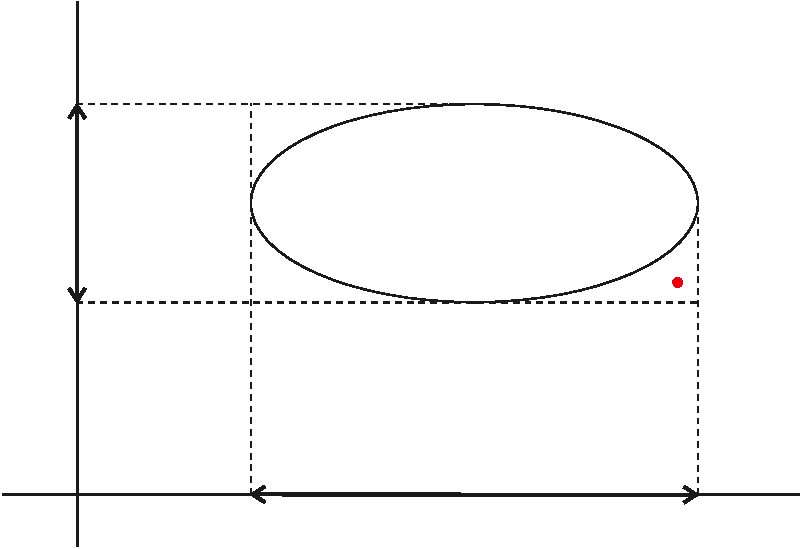
\includegraphics[width = 13cm]{pictures/picture_3_F.pdf}};
	    \draw [color = red](5.0,0.0) node[anchor = north west] { $(x_{01},x_{02})$ };
	    \draw [color = black](-5.9,4.2) node[anchor = north west] { $x_2$ };
	    \draw [color = black](5.5,-3.7) node[anchor = north west] { $x_1$ };
	     \draw [color = black](-1.0,1.4) node[anchor = north west] { $\text{společný obor dat } (x_1, x_2)$ };
	     \draw [color = black](-0.0,-3.6) node[anchor = north west] { $\text{obor hodnot } x_1$ };
	     \draw [color = black](-8.4,1.4) node[anchor = north west] { $\text{obor hodnot } x_2$ };
	    \end{tikzpicture}
	    \caption{ $(x_{01},x_{02})$ leží uvnitř oboru hodnot pro~obě $x_1$ i~$x_2$ ale vně společného oboru původních dat.}
	\end{figure}
\end{itemize}
\end{remark}
\end{description}
